\documentclass{article}
\usepackage[utf8]{inputenc}
\usepackage{graphicx}
\graphicspath{ {./grafici/} }
\usepackage{placeins}

\title{Alberi Binari vs Alberi Rosso-Neri: ricerca ed inserimento}
\author{Marco Vignozzi}

\begin{document}

\maketitle

\section{Introduzione}
In questo esperimento analizzo le prestazioni di Alberi Binari di Ricerca e Alberi Rosso-Neri nell'inserimento di un numero crescente di valori, e nella ricerca su un numero crescente di valori, per poi confrontare i risultati ottenuti attraverso dei grafici.

\section{Caratteristiche teoriche}
Di seguito introduco le caratteristiche teoriche delle strutture dati e degli algoritmi utilizzati, con riferimento alle prestazioni attese.

\subsection{Alberi Binari di Ricerca (ABR)}
\begin{itemize}
    \item \textbf{Struttura Dati}
\end{itemize}
Gli ABR sono degli alberi in cui ogni nodo ha al massimo due figli e tutti i valori nel sottoalbero sinistro di ciascun nodo sono minori o uguali al valore del nodo, mentre tutti quelli nel sottoalbero destro sono maggiori. La struttura degli ABR mantiene il valore del nodo iniziale (radice) e ciascun nodo ha come attributi un valore e tre puntatori, due ai nodi figli (destro e sinistro) e uno al nodo padre.
\begin{itemize}
    \item \textbf{Algoritmi}
\end{itemize}
Gli algoritmi di Ricerca e Inserimento vengono eseguiti in un Tempo O(h) dove h è l'altezza dell'albero.

\subsection{Alberi Rosso-Neri (ARN)}
\begin{itemize}
    \item \textbf{Struttura Dati}
\end{itemize}
Gli ARN hanno la struttura degli ABR ma con l'aggiunta di un attributo: il colore del nodo, rosso o nero. Ogni foglia dell'albero ha come figli dei nodi speciali chiamati NIL. Un ARN deve soddisfare le seguenti proprietà:
\begin{enumerate}
    \item Ogni nodo è rosso o nero.
    \item La radice è nera.
    \item Ogni foglia è nera (intesa come foglia terminale NIL).
    \item Se un nodo è rosso, allora entrambi i suoi figli sono neri.
    \item Per ogni nodo, tutti i cammini semplici che vanno dal nodo alle foglie sue discendenti contengono lo stesso numero di nodi neri.
\end{enumerate}
Grazie a queste proprietà un ARN con n nodi ha la caratteristica di avere un'altezza massima di $2{\log_{2}{(n+1)}}$.
\begin{itemize}
    \item \textbf{Algoritmi}
\end{itemize}
Gli algoritmi di Ricerca e Inserimento per un ARN con n nodi vengono eseguiti in un tempo O(${\log_{2}{n}}$).

\subsection{Prestazioni teoriche}
\begin{itemize}
    \item \textbf{Inserimento}
\end{itemize}
Nel caso migliore l'ABR è perfettamente bilanciato e il tempo di esecuzione dell'algoritmo di Inserimento élo stesso sia per ABR che per ARN, quindi O(${\log_{2}{n}}$). \\
Nel caso peggiore però l'ABR è equivalente a una lista e per ogni Inserimento si dovrà scorrere tutta la lista, rendendo il tempo di esecuzione un O(n) per l'ABR contro l'O(${\log_{2}{n}}$)  dell'ARN.

\begin{itemize}
    \item \textbf{Ricerca}
\end{itemize}
In questo caso i tempi di esecuzione dipendono da più fattori: la presenza del valore cercato, la sua posizione e dalla struttura assunta dall'albero nel caso di ABR. Nel caso peggiore dovremo scorrere tutto l'albero per trovare (o non trovare) il valore obiettivo. Di conseguenza i tempi saranno gli stessi del caso dell'inserimento sia per ABR che per ARN.

\section{Codice}
\subsection{Moduli}
Moduli esterni:
\begin{itemize}
    \item \textbf{random}
    \item \textbf{matplotlib.pyplot}
    \item \textbf{timeit}
    \item \textbf{pathlib}
\end{itemize}
Moduli propri:
\begin{enumerate}
    \item \textbf{BTclass.py}: in questo modulo è contenuta la struttura dati ABR e tutti i suoi metodi.
    \item \textbf{RBTclass.py}: qui troviamo struttura e metodi per l'ARN.
    \item \textbf{test.py}: questo modulo si occupa dello svolgimento dei test e contiene metodi per la generazione dei documenti. Utilizza \verb|BTclass.py|, \verb|RBTclass.py| e tutti i moduli esterni.
    \item \textbf{main.py}: in questo modulo si creano i test e si richiede di stampare i documenti richiesti. Utilizza il modulo \verb|test.py|. 
\end{enumerate}

\subsection{Classi}
Vengono utilizzate le seguenti classi:
\begin{itemize}
    \item \textbf{Node}: questa classe è presente nei moduli 1 e 2 e contiene la struttura del nodo del relativo albero.
    \begin{itemize}
        \item Nel nodo dell'ABR non è presente l'attributo \emph{parent} che non è necessario visto che ricerca e inserimento sono implementate in maniera ricorsiva. 
        \item Nel nodo dell'ARN sono presenti anche gli attributi \emph{parent} e \emph{color}.
    \end{itemize}
    \item \textbf{BTclass}: struttura dati per ABR con metodi per inserimento e ricerca, oltre a un metodo per la stampa. Mantiene il nodo radice nell'attributo \emph{root}.
    \item \textbf{RBTclass}: struttura dati per ARN anch'essa con metodi per inserimento, ricerca e stampa.
    \item \textbf{Test}: questa è la classe principale. Quando viene istanziata genera i test richiesti (vengono eseguiti \emph{(end-start)/step} test per tipo) e li salva nell'attributo \emph{tests}, una lista di tuple dove ciascuna rappresenta un test:\\(tipo albero, tipo test, elementi cercati/inseriti, tempo impiegato).\\Il costruttore richiede di specificare i seguenti parametri:
    \begin{itemize}
        \item \emph{t\_type}: determina l'ordinamento con cui viene creata la lista di numeri da inserire negli alberi. Può essere \emph{"random"}(default) per ordinamento casuale o qualsiasi altra stringa per ordinamento sequenziale.
        \item \emph{r\_type}: determina il tipo di ricerca e può essere \emph{"success"}(default) per ricerca con successo o qualsiasi altro valore per ricerca senza successo.
        \item \emph{start}: valore minimo del numero di elementi cercati/inseriti in un test. 1 è il valore di default.
        \item \emph{max\_value}: valore massimo del numero di elementi cercati/inseriti in un test. 10 è il valore di default.
        \item \emph{step}: distanza tra il numero di elementi cercati/inseriti in un test e il successivo. 1 è il valore di default.
        \item \emph{dir\_name}: nome della cartella in cui viene salvata la documentazione (a partire dal percorso \emph{./doc}). "test" è il valore di default.
    \end{itemize}
\end{itemize}

\subsection{Metodi}
\begin{itemize}
    \item \textbf{Modulo BTclass.py}
\end{itemize}
\begin{verbatim}get_name(self)\end{verbatim}
Restituisce la stringa \emph{"binary tree"}.
\begin{verbatim}clear(self)\end{verbatim}
Cancella l'albero settando \emph{root} a \emph{None}.
\begin{verbatim}set_root(self, key)\end{verbatim}
Assegna il valore \verb|key| alla radice dell'albero come \verb|Node(key)|.
\begin{verbatim}insert(self, key)\end{verbatim}
Riceve un valore \verb|key| da inserire nell'albero e lo passa al metodo di inserimento insieme al nodo iniziale \emph{root}.
\begin{verbatim}insert_node(self, current_node, key)\end{verbatim}
Metodo di inserimento. Riceve il nodo corrente \verb|current_ node| e il valore \verb|key| da inserire. Trova il posto giusto in maniera ricorsiva e lo inserisce come \verb|Node(key)|.
\begin{verbatim}find(self, key)\end{verbatim}
Passa il valore \verb|key| alla routine di ricerca, oltre all'attributo \emph{root} come nodo iniziale.
\begin{verbatim}find_node(self, current_node, key)\end{verbatim}
Metodo di ricerca. Riceve il nodo corrente \verb|current_node| e un valore \verb|key| e lo cerca nell'albero in maniera ricorsiva, ritornando \emph{True} se il valore è presente in uno dei nodi, altrimenti \emph{False}.
\begin{verbatim}inorder(self)\end{verbatim}
Stampa in ordine crescente i valori contenuti nell'albero.\\

\begin{itemize}
    \item \textbf{Modulo RBTclass.py}
\end{itemize}
\begin{verbatim}get_name(self)\end{verbatim}
Ritorna la stringa \emph{"red-black tree"}.
\begin{verbatim}clear(self)\end{verbatim}
Cancella l'albero settando \emph{root} a \emph{None}.
\begin{verbatim}set_root(self, node)\end{verbatim}
Riceve un nodo \verb|node| e lo assegna alla radice \emph{root}.
\begin{verbatim}insert(self, key)\end{verbatim}
Riceve un valore \verb|key| da inserire nell'albero e lo passa al metodo di inserimento come \emph{Node(key)} insieme al nodo iniziale \emph{root}.
\begin{verbatim}left_rotate(self, x)\end{verbatim}
Riceve il nodo \verb|x| intorno al quale far girare l'albero.
\begin{verbatim}right_rotate(self, x)\end{verbatim}
Riceve il nodo \verb|x| intorno al quale far girare l'albero.
\begin{verbatim}insert_node(self, z)\end{verbatim}
Metodo di inserimento. Riceve il nodo \verb|z| da inserire, trova il posto giusto e lo inserisce per poi richiamare il metodo di fixup.
\begin{verbatim}rb_insert_fixup(self, z)\end{verbatim}
Riceve il nodo \verb|z| da cui iniziare il fixup e riordina i colori dei nodi dell'albero in modo che rispettino le regole per l'albero rosso nero.
\begin{verbatim}find(self, key)\end{verbatim}
Passa il valore \verb|key| alla routine di ricerca, passandole \emph{root} come nodo iniziale.
\begin{verbatim}find_node(self, current_node, key)\end{verbatim}
Metodo di ricerca. Riceve il nodo corrente \verb|current_node| e un valore \verb|key| e lo cerca nell'albero in maniera ricorsiva, ritornando \emph{True} se il valore è presente in uno dei nodi, altrimenti \emph{False}.
\begin{verbatim}inorder(self)\end{verbatim}
Stampa in ordine crescente i valori contenuti nell'albero.\\

\begin{itemize}
    \item \textbf{Modulo test.py}
\end{itemize}
\begin{verbatim}random_list(n)\end{verbatim}
Riceve un valore \verb|n| intero e restituisce una lista di interi nel range da 0 a \verb|n| ordinati in maniera casuale.
\begin{verbatim}create_tests_list(op, n_list, start, end, step)\end{verbatim}
Lista parametri:
\begin{itemize}
    \item \verb|op|: una stringa che specifica il test da eseguire (\emph{"find"} per la ricerca con successo e \emph{"insert"} per l'inserimento, o un'altra stringa per la ricerca senza successo).
    \item \verb|n_list|: una lista di valori che vengono usati per inizializzare gli alberi per la ricerca.
    \item \verb|start|: valore minimo di elementi cercati/inseriti in un test.
    \item \verb|end|: valore massimo di elementi cercati/inseriti in un test.
    \item \verb|step|: differenza tra il numero di elementi cercati/inseriti da un test al successivo.
\end{itemize}
Questo metodo istanzia gli alberi necessari al test e richiama i metodi \verb|test_insert()| o \verb|test_find()| (a seconda del valore di \verb|op|) un numero \emph{(end-start)/step} di volte, aggiungendo ad ogni iterazione il risultato del test eseguito a una lista di tuple che verrà usata come valore di ritorno. Ogni elemento della lista contiene le seguenti informazioni riguardo a un test eseguito: (tipo albero, tipo test, elementi cercati/inseriti, tempo impiegato).
\begin{verbatim}test_insert(tree, values_list, number_of_entries, r=0)\end{verbatim}
Questo metodo effettua il numero di inserimenti richiesti attraverso il parametro \verb|number_of_entries| nell'albero \verb|tree| prendendo gli elementi dalla \verb|values_list|. Viene calcolato il tempo necessario a inserire tutti gli elementi. Il metodo ritorna una lista di tuple che rappresenta il test eseguito.\\
Questo metodo è utilizzato anche per creare gli alberi su cui effettuare i test di ricerca. In base al tipo di ricerca che vorremo eseguire passeremo il parametro \verb|r| settato a 0 (ricerca con successo) o a 1 (ricerca senza successo). 
\begin{verbatim}test_find(tree, values_list, number_of_searches, r=0)\end{verbatim}
Questo metodo effettua il numero di ricerche richieste dal parametro \verb|number_of_searches| nell'albero \verb|tree| cercando gli elementi nella \verb|values_list|. Il parametro \verb|r| serve in questo caso a definire il tipo di ricerca: \\
\verb|for x in range(1, number_of_searches, r+1):|\\
\verb|   tree.find(values_list[x])|\\
Con \verb|r=0| effettuerà la ricerca con successo, cercando gli stessi elementi della \verb|values_list| che erano stati inseriti. \\
Con \verb|r=1| effettuerà la ricerca senza successo, cercheremo elementi diversi.\\
Viene calcolato il tempo necessario a cercare tutti gli elementi. Il metodo ritorna la lista di tuple che rappresenta il test eseguito, con la stessa struttura di quella ritornata da \verb|test_insert()|.
\begin{verbatim}get_values_list(value_type, op_type, tree_type, tests_list)\end{verbatim}
Questo metodo estrae una lista di valori dalla lista di tuple \verb|tests__list| e la ritorna. Il valore estratto è definito attraverso i parametri \verb|value_type|, \verb|op_type| e \verb|tree_type|, che permettono di scegliere: valore da estrarre (elementi cercati/inseriti o tempo impiegato), per quale tipo di operazione (inserimento o ricerca, con o senza successo) e per quale tipo di albero. Utilizza una routine di appoggio \verb|choose_value()|.
\begin{verbatim}choose_value(test_element, value_type)\end{verbatim}
Riceve una tupla \verb|test_element| che rappresenta un test e il tipo di valore da estrarre \verb|value_type|. Ritorna il valore scelto che può essere il tempo impiegato (\emph{"time"}) o il numero di elementi cercati/inseriti in quel test (qualsiasi altra stringa). 
\begin{verbatim}create_plot(self)\end{verbatim}
Metodo della classe che serve a generare i grafici degli esperimenti.
\begin{verbatim}create_docs(self)\end{verbatim}
Metodo della classe che genera i file di testo nella cartella specificata al momento della creazione del test.

\section{Esperimenti}
I seguenti esperimenti sono stati condotti su un computer portatile HP envy con caratteristiche: CPU AMD Ryzen 7 5700U 1.80 GHz, scheda video integrata Radeon Graphics e 16GB di RAM.
\begin{enumerate}
    \item Inserimento e ricerca con successo di un numero crescente di elementi con lista di valori non ordinata.
    \item Inserimento e ricerca senza successo di un numero crescente di elementi con lista di valori non ordinata.
    \item Inserimento e ricerca con successo di un numero crescente di elementi con lista di valori ordinata.
\end{enumerate}

\subsection{Esperimento 1}
\subsubsection{Descrizione}
In questo esperimento vengono eseguiti 44 test di inserimento e 44 di ricerca, dove vengono inseriti/cercati dai 1000 ai 9800 valori con step di 200. La lista dei valori inseriti negli alberi viene generata all'interno del metodo \verb|random_list(n)| (con \emph{n=9800}) in questo modo:
\begin{verbatim}
r_list = list(range(n))
random.shuffle(r_list)
\end{verbatim}
Vengono costruiti gli alberi con questa lista e poi si eseguono i test di inserimento e di ricerca.\\
Per ognuno dei 45 test di inserimento viene misurato il tempo all'interno del metodo \verb|test_insert(tree, values_list, number_of_entries, r=0)| per la porzione di codice:
\begin{verbatim}
start = timer()
for x in range(0, number_of_entries, r+1):
    tree.insert(values_list[x])
end = timer()
\end{verbatim}
Per ognuno dei 45 test di ricerca viene misurato il tempo all'interno del metodo \verb|test_find(tree, values_list, number_of_searches, r=0)| per la porzione di codice:
\begin{verbatim}
start = timer()
for x in range(1, number_of_searches, r+1):
    tree.find(values_list[x])
end = timer()
\end{verbatim}
I valori così ottenuti sono usati per creare i grafici 1 e 2 in Figura \ref{fig:1}. Qui vengono confrontati i tempi di inserimento per ABR e ARN, e quelli di ricerca.
\subsubsection{Prestazioni attese}
La lista \verb|values_list| è implementata in python come un array dinamico, quindi la stima asintotica del tempo di accesso a un elemento è O(1). Abbiamo un ciclo \emph{for} all'interno del quale vengono eseguiti \verb|tree.find()| o \verb|tree.insert()| \emph{r} volte, dove \emph{r} è il numero di elementi cercati o inseriti in un test (\emph{1000 < r < n}). Di conseguenza la stima asintotica del tempo di esecuzione della parte di codice misurata è O(${r\log_{2}{n}}$) per l'ARN e O(${r\log_{2}{h}}$) per l'ABR, dove \emph{h} è l'altezza dell'albero.
\subsubsection{Analisi}
Il grafico in Figura \ref{fig:1} mostra come ABR e ARN abbiano prestazioni simili nell'inserimento non ordinato di valori con tempi massimi di 0.0329s per ARN, contro i 0.0368s dell'ABR (la presenza di picchi potrebbe essere dovuta a conflitti con il sistema operativo). Nella ricerca si nota invece una maggiore distanza nei tempi di esecuzione, dove l'ARN risulta migliore. L'ARN impiega un tempo massimo di 0.0268s contro i 0.0338s dell'ABR. Questo è dovuto alla presenza di nodi a profondità maggiore nell'ABR, laddove invece l'ARN si mantiene sempre bilanciato.

\subsection{Esperimento 2}
\subsubsection{Descrizione}
In questo esperimento si esegue lo stesso numero di test dell'esperimento 1 e sullo stesso numero di elementi, ma si ricercano valori che non sono stati inseriti negli alberi. Vengono effettuate le stesse misurazioni con gli stessi metodi.\\
I valori così ottenuti servono a creare il grafico 3 in Figura \ref{fig:1} e i grafici in Figura \ref{fig:2}. Nel primo il confronto è effettuato sui tempi di ricerca senza successo per ABR e ARN. In Figura \ref{fig:2} si confrontano i tempi di ricerca con e senza successo su una stessa struttura dati.
\subsubsection{Prestazioni attese}
Le prestazioni attese a livello teorico sono le stesse dell'esperimento 1, ma nel caso peggiore ci aspettiamo qualche peggioramento dovuto al dover sempre percorrere l'albero fino alle foglie.
\subsubsection{Analisi risultati}
I risultati ottenuti mostrano che i tempi di esecuzione nel caso di ricerca senza successo sono sempre maggiori del caso di ricerca con successo. Questo risultato non è ovvio per l'ABR, dove la durata della ricerca dipende dall'altezza del sottoalbero ispezionato. Anche in questo caso l'ABR ha prestazioni peggiori con un tempo massimo di 0.0388s contro i 0.0310s dell'ARN. Anche stavolta (come nell'esperimento 1) la discrepanza è dovuta alla maggiore profondità delle foglie rispetto all'ARN.
\subsection{Esperimento 3}
\subsubsection{Descrizione}
In questo esperimento vengono eseguiti 79 test di inserimento e 79 di ricerca, dove vengono inseriti/cercati da 1 a 791 valori con step di 10. La lista dei valori inseriti negli alberi viene generata direttamente nel costruttore della classe \verb|Test| in questo modo:
\begin{verbatim}
numbers_list = list(range(max_value))
\end{verbatim}
dove \verb|max_value=800|. Vengono effettuate le stesse misurazioni con gli stessi metodi usati negli esperimenti 1 e 2. I valori ottenuti servono a creare i grafici in figura \ref{fig:3} che mostrano il confronto tra le due strutture sui tempi di esecuzione di inserimento e ricerca.\\
NOTA: ho scelto un valore più basso di elementi da inserire visto che con un numero troppo elevato il programma non veniva eseguito, perchè si effettuavano una quantità eccessiva di chiamate ricorsive ai metodi \verb|find()| e \verb|insert()| dell'ABR.
\subsubsection{Prestazioni attese}
Le prestazioni attese per l'ARN sono le stesse dell'esperimento 1 ovvero O(${n\log_{2}{n}}$), con \emph{n} numero elementi inseriti. Per quanto riguarda l'ABR stavolta l'inserimento è ordinato, di conseguenza ci si aspetta un tempo di esecuzione O(${n^2}$).
\subsubsection{Analisi risultati}
Questo esperimento evidenzia i limiti dell'ABR negli algoritmi di ricerca e inserimento. Infatti i tempi peggiorano notevolmente (rispetto all'esperimento 1) per l'ABR per cui si riesce ad apprezzare l'andamento esponenziale dei grafici in Figura \ref{fig:3}. L'ARN mantiene invece un andamento pressochè inalterato rispetto agli altri esperimenti. I tempi massimi sono molto più distanti: per l'inserimento otteniamo 0.0029s per l'ARN contro i 0.0619s dell'ABR, per la ricerca 0.0015s per l'ARN contro i 0.0689s dell'ABR.

\begin{figure}[hb]
    \centering
    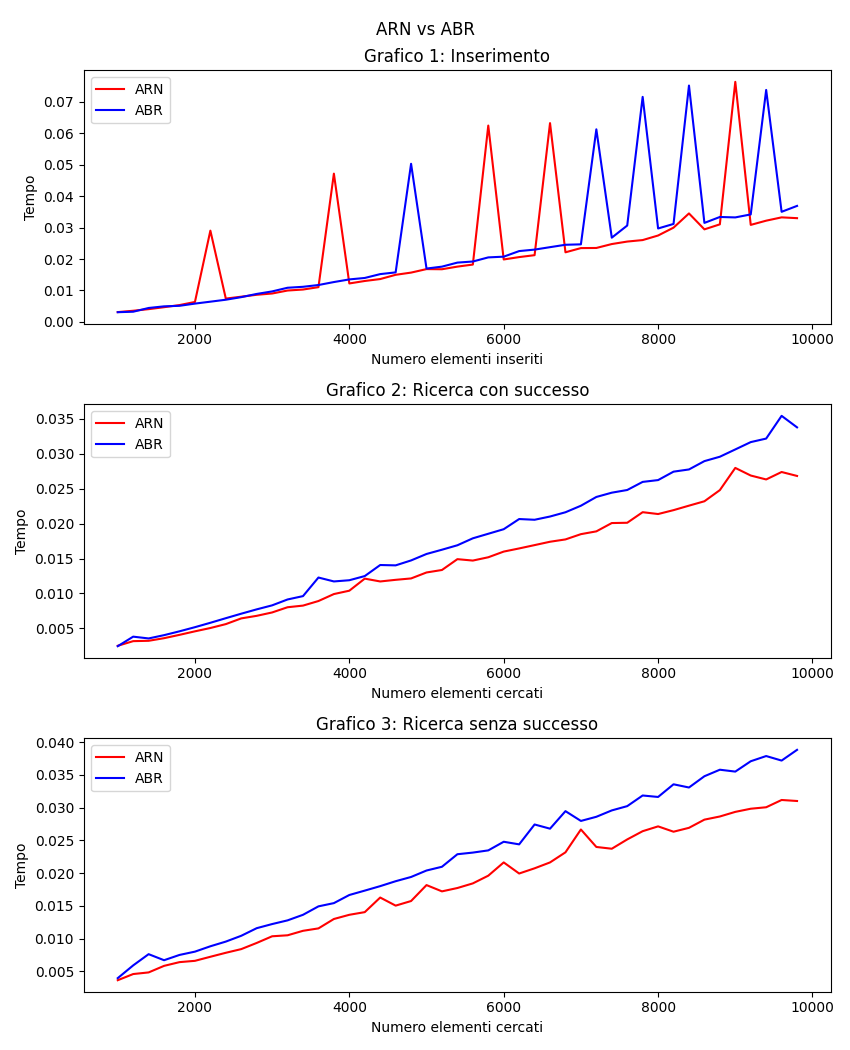
\includegraphics[height=8cm]{grafici/insert_and_search_comparison.png}
    \caption{questi grafici mostrano i risultati del confronto tra ARN e ABR per quanto riguarda i tempi di esecuzione }
    \label{fig:1}
\end{figure}
\begin{figure}[h]
    \centering
    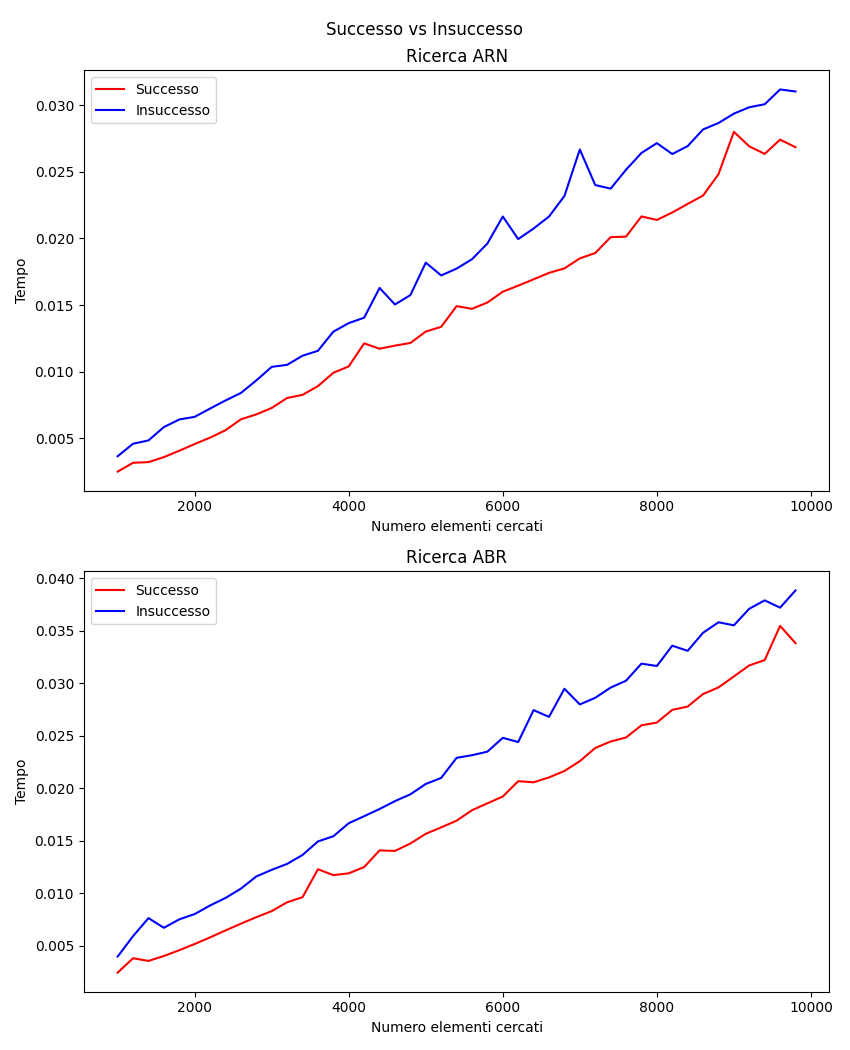
\includegraphics[height= 8cm]{grafici/sux_vs_notsux_comparison.png}
    \caption{questi grafici mostrano i risultati del confronto tra ricerca con successo e senza successo per uno stesso albero}
    \label{fig:2}
\end{figure}
\begin{figure}[h]
    \centering
    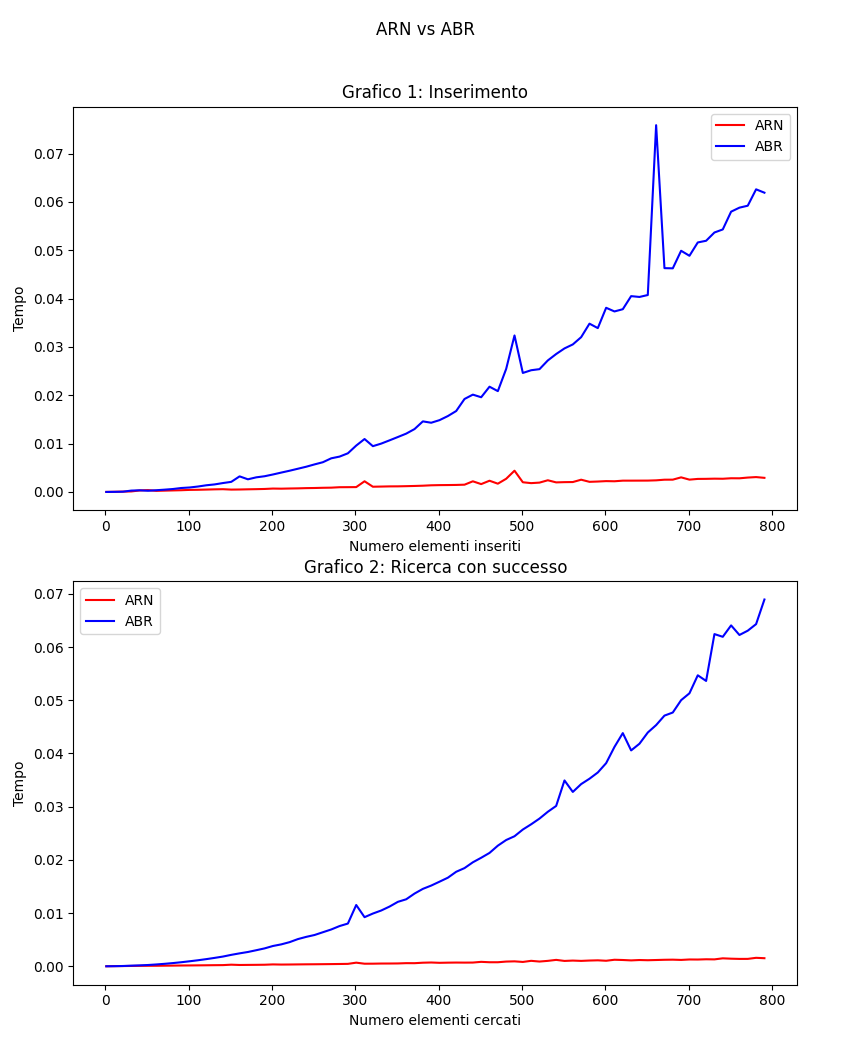
\includegraphics[height= 8cm]{grafici/ordered_insert_and_search_comparison.png}
    \caption{questi grafici mostrano i risultati del confronto tra ricerca con successo e senza successo per uno stesso albero}
    \label{fig:3}
\end{figure}

\FloatBarrier
\section{Conclusioni}
I risultati ottenuti in questi esperimenti sono fedeli a quelli teorizzati e mostrano come l'ARN sia decisamente migliore nei casi in cui si richiede inserimento di valori ordinati. L'ABR dal canto suo presenta una struttura più semplice, ma resta inferiore all'ARN anche nel caso in cui i valori inseriti non siano ordinati.\\ Una struttura ad ABR risulta quindi indicata solo nei casi in cui non ci sia bisogno di tanti nodi e soprattutto non si effettuino inserimenti ordinati, mentre l'ABR è sempre la scelta migliore.
\section{Dati utilizzati}
I dati utilizzati negli esperimenti sono presenti nei file di testo allegati. Essi contengono lista di valori utilizzata per poter duplicare l'esperimento e i tempi calcolati per ogni test.

\end{document}
